\documentclass[10pt]{beamer}

\usetheme{metropolis}
\usepackage{appendixnumberbeamer}
\usepackage{caption}

\usepackage{booktabs}
\usepackage[scale=2]{ccicons}

\usepackage{pgfplots}
\usepgfplotslibrary{dateplot}

\usepackage{xspace}
\usepackage{chronology}
\usepackage{tabls}
\usepackage{tikz}
\usepackage{bchart}
\usepackage{appendixnumberbeamer}

\newcommand{\themename}{\textbf{\textsc{metropolis}}\xspace}

\hypersetup{pdfpagemode=FullScreen}

\title{Linux}
\subtitle{Eine kurze Einführung}
\date{20. Mai 2019}
\author{Alex Neher}
\titlegraphic{\hfill
\includegraphics[height=1.5cm]{img/Tux.png}}

\begin{document}

\pagestyle{empty}
	
\begin{frame}

\end{frame}

\maketitle

\begin{frame}{Inhalt}
  \setbeamertemplate{section in toc}[sections numbered]
  \tableofcontents[hideallsubsections]
\end{frame}

\section{Was ist Linux?}

\begin{frame}{Was ist Linux?}
    \begin{itemize}[<+- | alert@+>]
        \item Betriebssystem/Kernel
        \item Meist verwendet für Server
        \item Android
    \end{itemize}

\end{frame}

\begin{frame}{Betriebssystem/Kernel}
    \centering
    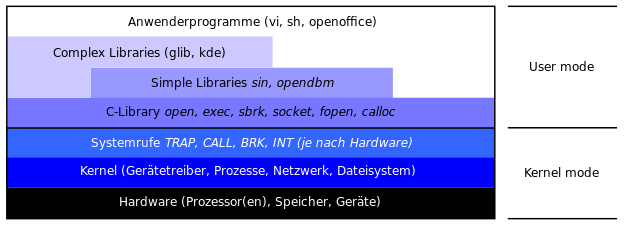
\includegraphics[keepaspectratio,width=0.9\textwidth]{img/kernel_schichten.png}
\end{frame}

\section{Geschichte}
\begin{frame}{Linus Torvalds}
	\begin{columns}
		 \column{0.50\textwidth}
		 	\begin{itemize}[<+- | alert@+>]
		 		\item Finnischer Informatikstudent
		 		\item Wollte Dinge mit seinem UNIX-Computer machen, die nicht unterstützt wurden
		 		\item Entschied sich, diese Dinge selbst zu programmieren
		 		\item Programmierte schlussendlich sein eigenes Betriebssystem
		 		\item Vorsitzender der Linux-Foundation
		 	\end{itemize}
	 	\column{0.50\textwidth}
	 		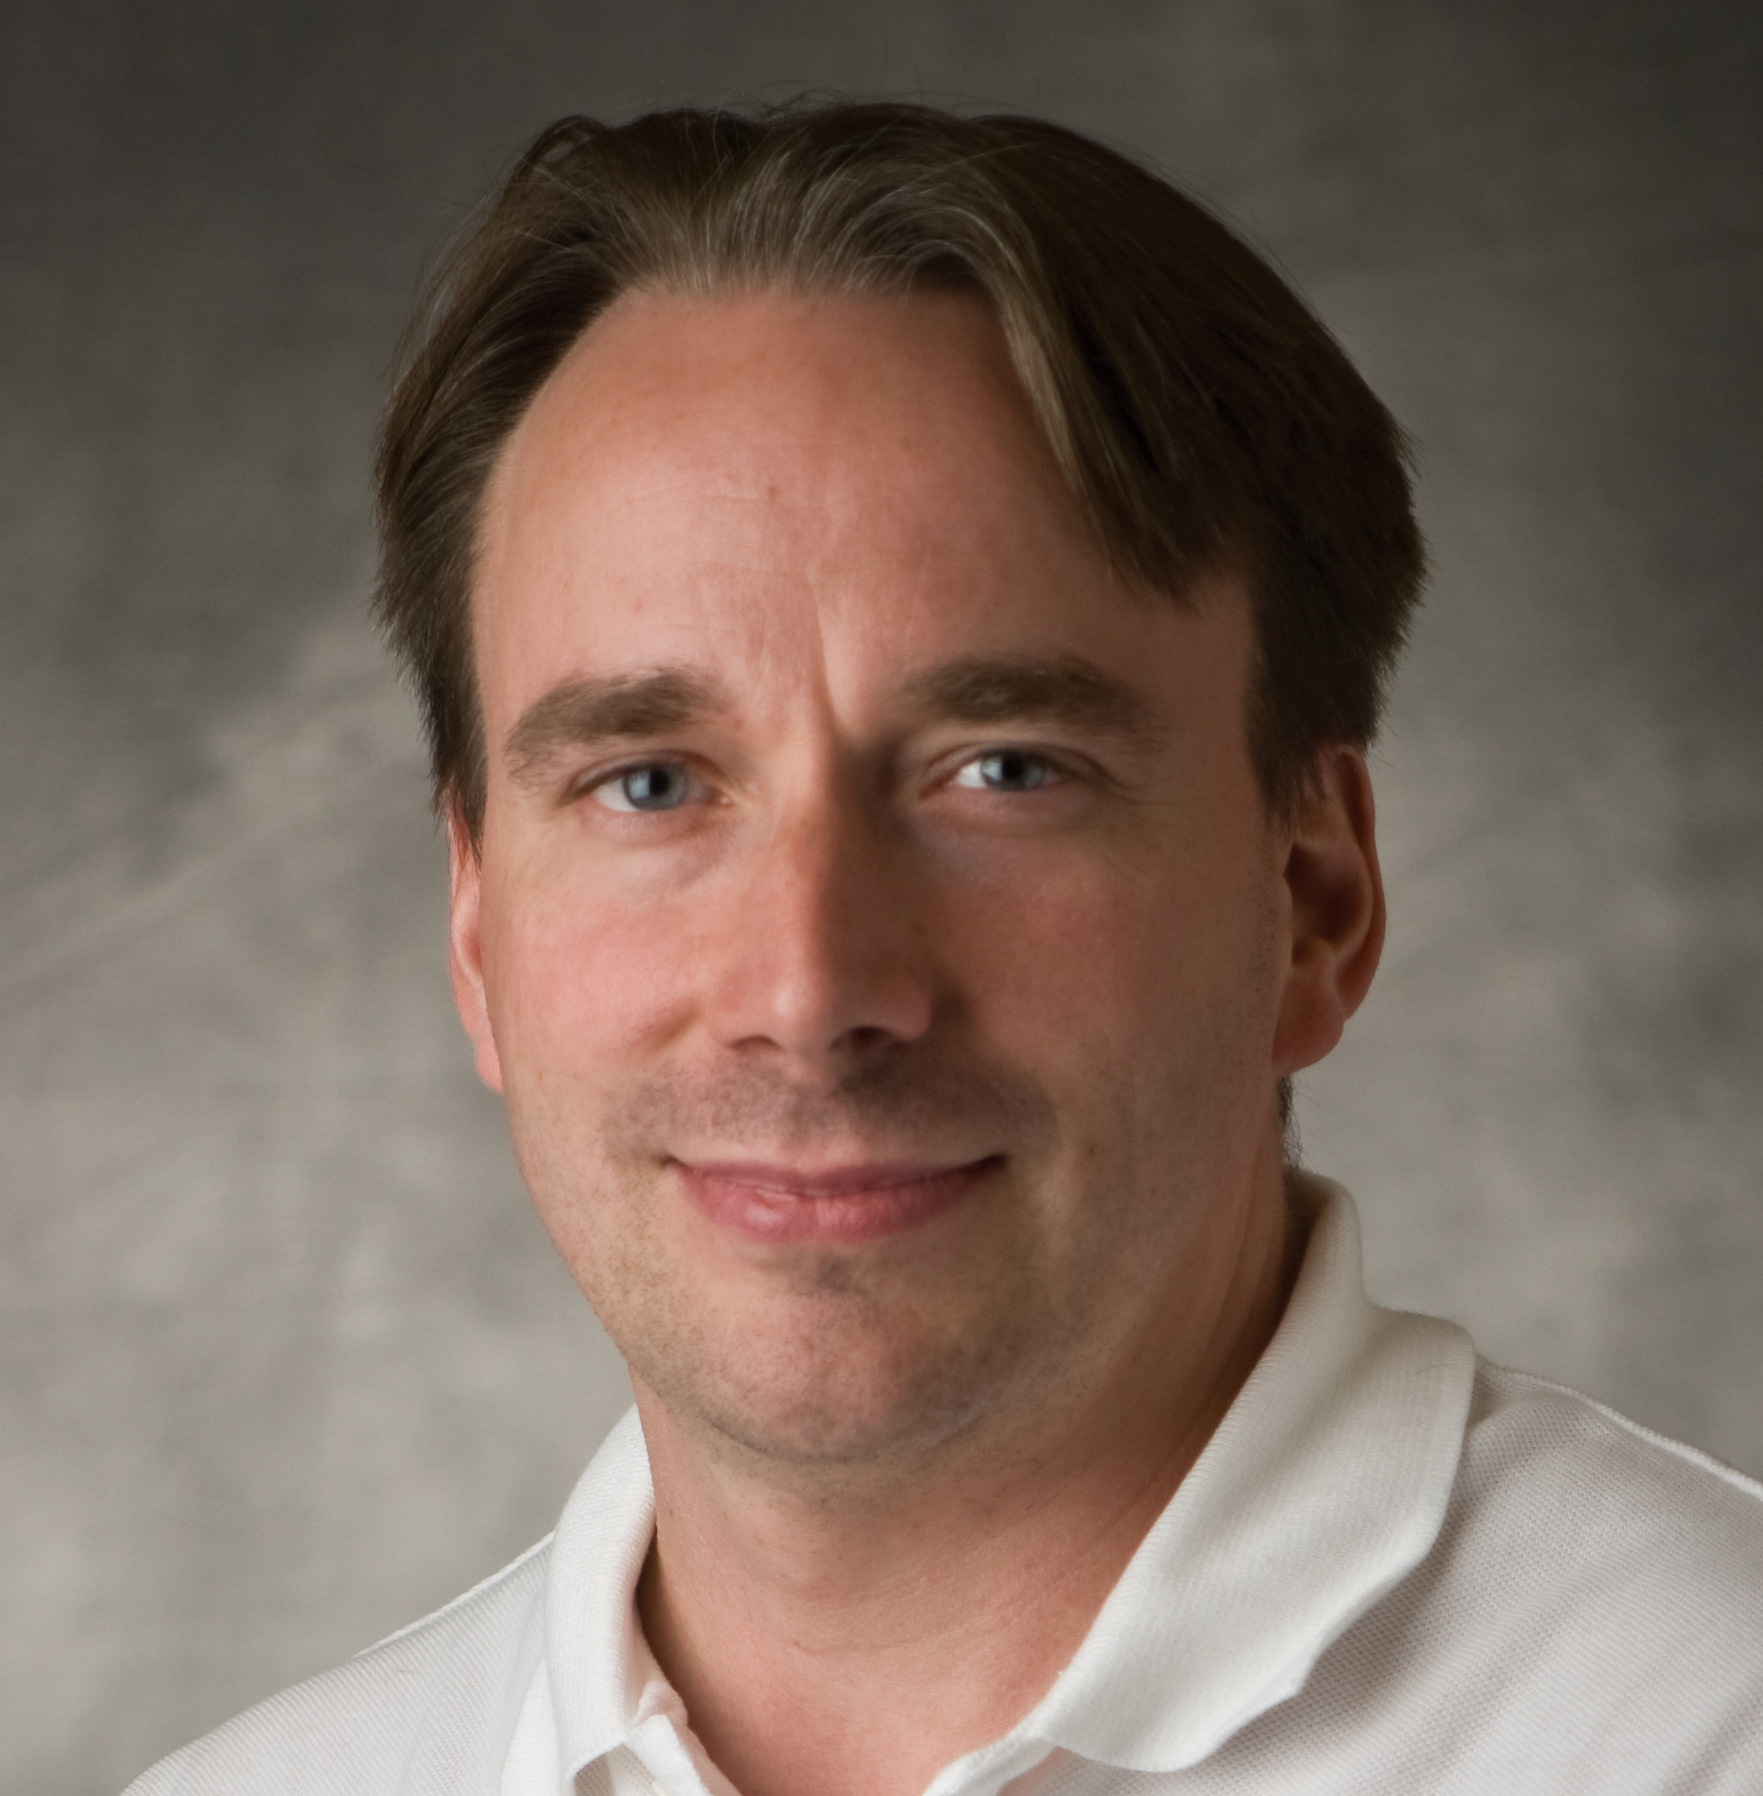
\includegraphics[scale=0.25]{img/torvalds.png}
	\end{columns}
\end{frame}

\section{Open Source}

\begin{frame}{Was ist Open Source?}
	\begin{itemize}[<+- | alert@+>]
		\item Der Code des Programms ist öffentlich verfügbar
		\item Jeder kann den Code lesen, verstehen und auf allfällige Fehler/Schwachstellen überprüfen
		\item Jeder kann den Code seinen Bedürfnissen anpassen und Fehler beheben
	\end{itemize}
\end{frame}

\begin{frame}{Open Source und Sicherheit/Privatsphäre}
	\begin{itemize}[<+- | alert@+>]
		\item Jeder kann den Code auf allfällige Backdoors überprüfen
		\item Falls zu viel 'nach Hause telefoniert' wird, kann man das einfach anpassen
		\item Schwachstellen werden schnell gefunden und behoben
	\end{itemize}
\end{frame}

\section{Linux heute}

\begin{frame}{Distributionen}
    \centering
    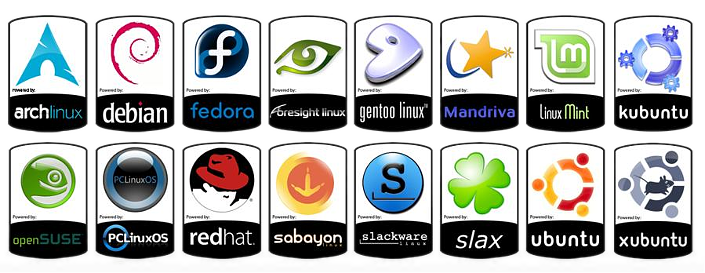
\includegraphics[keepaspectratio,width=0.9\textwidth]{img/logos_2.png}
\end{frame}

\begin{frame}{Marktanteil Webserver}
    \begin{centering}
	\begin{bchart}[step=10,max=100]
		\bcbar[text=Linux]{69.9}
			\smallskip
		\bcbar[text=Windows]{30.1}
	\end{bchart}
\end{centering}
    
    Verteilung der Betriebssysteme auf den Webservern der top 10 Millionen Websiten
\end{frame}

\begin{frame}{Marktanteil IoT}
\begin{figure}
	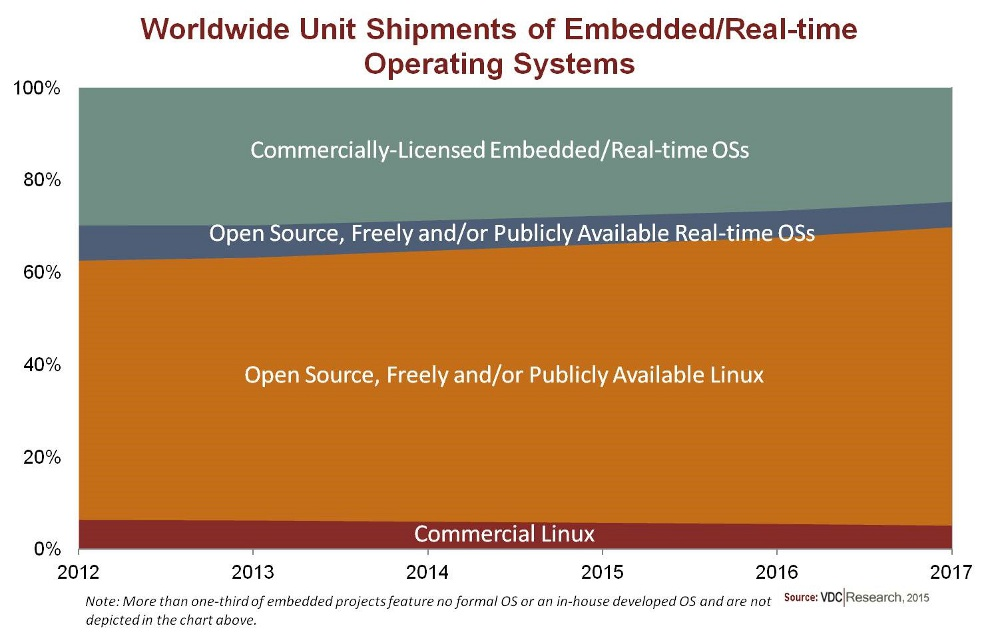
\includegraphics[keepaspectratio,
	width=0.9\textwidth]{img/iot.jpg}
\end{figure}
\end{frame}


\begin{frame}{Marktanteil Desktop/Laptop}
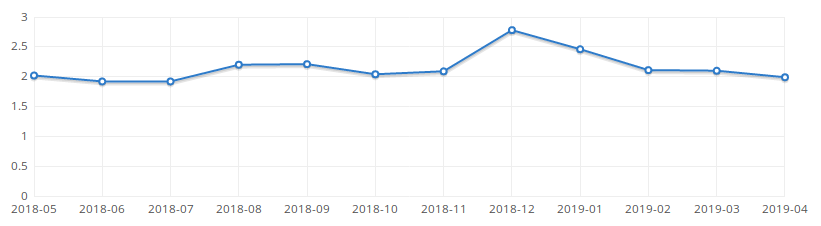
\includegraphics[keepaspectratio, width=0.9\textwidth]{img/market_share.png}
\end{frame}

\begin{frame}{Marktanteil Desktop/Laptop}
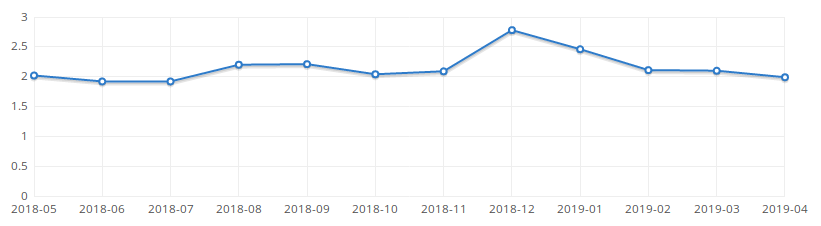
\includegraphics[keepaspectratio, width=0.9\textwidth]{img/market_share.png}

\centering
\begin{table}
\begin{tabular}{l|c}
	\toprule
	\textbf{Betriebssystem} & \textbf{Marktanteil} \\
	\hline
	Windows & 87.4\% \\
	MacOS & 9.7\% \\
	Linux & 2.2\% \\
	ChromeOS & 0.33\% \\
	BSD & 0.01\% \\
	\bottomrule
\end{tabular}
\end{table}	
\end{frame}

\begin{frame}{Desktopumgebungen}
\centering
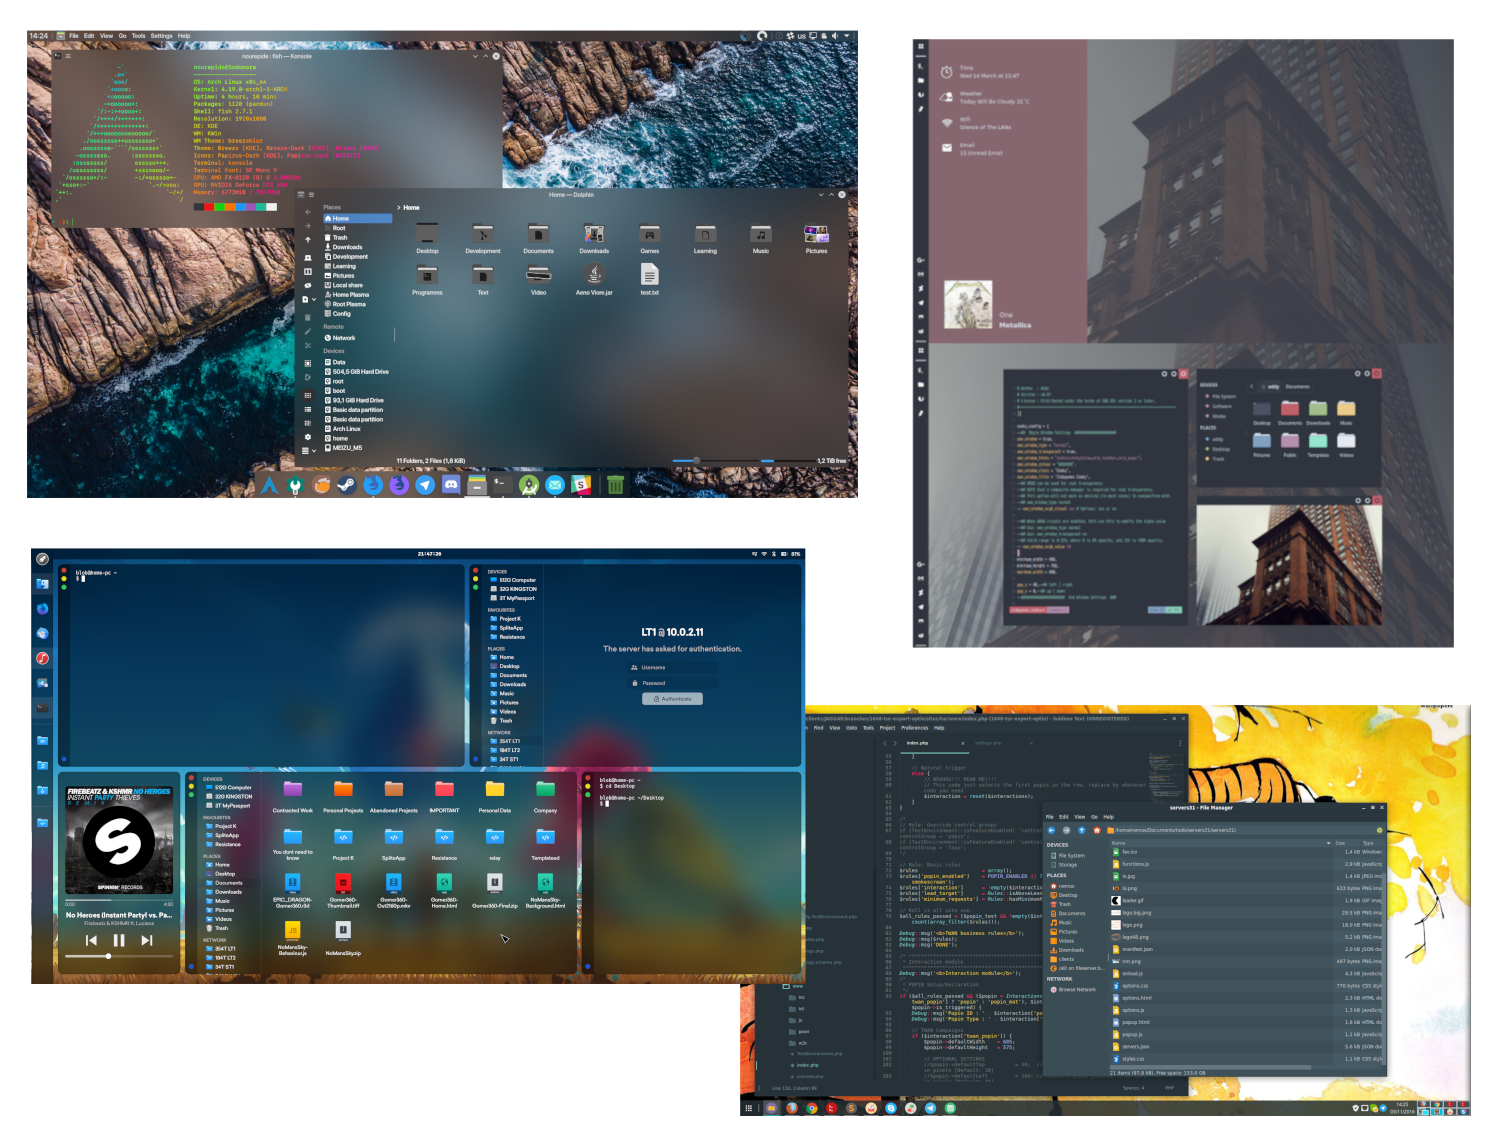
\includegraphics[keepaspectratio,width=0.9\textwidth]{img/desktops.png}
\end{frame}

\begin{frame}[standout]
Fragen?
\end{frame}

\end{document}
